%%
%% This is file `sample-sigconf.tex',
%% generated with the docstrip utility.
%%
%% The original source files were:
%%
%% samples.dtx  (with options: `sigconf')
%% 
%% IMPORTANT NOTICE:
%% 
%% For the copyright see the source file.
%% 
%% Any modified versions of this file must be renamed
%% with new filenames distinct from sample-sigconf.tex.
%% 
%% For distribution of the original source see the terms
%% for copying and modification in the file samples.dtx.
%% 
%% This generated file may be distributed as long as the
%% original source files, as listed above, are part of the
%% same distribution. (The sources need not necessarily be
%% in the same archive or directory.)
%%
%% The first command in your LaTeX source must be the \documentclass command.

\documentclass[sigconf]{acmart}
\usepackage{bm}
\usepackage{array}
\usepackage{float}
\usepackage{natbib}

%%
%% \BibTeX command to typeset BibTeX logo in the docs
\AtBeginDocument{%
  \providecommand\BibTeX{{%
    \normalfont B\kern-0.5em{\scshape i\kern-0.25em b}\kern-0.8em\TeX}}}

%% Rights management information.  This information is sent to you
%% when you complete the rights form.  These commands have SAMPLE
%% values in them; it is your responsibility as an author to replace
%% the commands and values with those provided to you when you
%% complete the rights form.
\setcopyright{acmcopyright}
\copyrightyear{2020}
\acmYear{2020}
\acmDOI{10.1145/1122445.1122456}

%% These commands are for a PROCEEDINGS abstract or paper.
\acmConference[SBES 2020]{SBES '2020: XXXIV BRAZILIAN SYMPOSIUM ON SOFTWARE ENGINEERING (SBES 2020)}{October 19--23, 2020}{Natal, Brazil}
\acmBooktitle{XXXIV BRAZILIAN SYMPOSIUM ON
SOFTWARE ENGINEERING (SBES 2020),
  October 19--23, 2020, Natal, Brazil}


%%
%% Submission ID.
%% Use this when submitting an article to a sponsored event. You'll
%% receive a unique submission ID from the organizers
%% of the event, and this ID should be used as the parameter to this command.
%%\acmSubmissionID{123-A56-BU3}

%%
%% The majority of ACM publications use numbered citations and
%% references.  The command \citestyle{authoryear} switches to the
%% "author year" style.
%%
%% If you are preparing content for an event
%% sponsored by ACM SIGGRAPH, you must use the "author year" style of
%% citations and references.
%% Uncommenting
%% the next command will enable that style.
%%\citestyle{acmauthoryear}

%%
%% end of the preamble, start of the body of the document source.
\begin{document}

%%
%% The "title" command has an optional parameter,
%% allowing the author to define a "short title" to be used in page headers.
\title{CoNCRA: A Convolutional Neural Networks Code Retrieval Approach}

%%
%% The "author" command and its associated commands are used to define
%% the authors and their affiliations.
%% Of note is the shared affiliation of the first two authors, and the
%% "authornote" and "authornotemark" commands
%% used to denote shared contribution to the research.
\author{Marcelo de Rezende Martins}
\email{rezende.martins@gmail.com}
\affiliation{%
\institution{IPT – Institute for Technological Research}
 \city{Sao Paulo}
 \state{Sao Paulo}
 \country{Brazil}
}


\author{Marco Aurélio Gerosa}
\email{marco.gerosa@nau.edu}
\affiliation{%
 \institution{Northern Arizona University (NAU)}
 \city{Flagstaff}
 \state{Arizona}
 \country{United States}
}

%%
%% By default, the full list of authors will be used in the page
%% headers. Often, this list is too long, and will overlap
%% other information printed in the page headers. This command allows
%% the author to define a more concise list
%% of authors' names for this purpose.


%%
%% The abstract is a short summary of the work to be presented in the
%% article.
\begin{abstract}
    Software developers search for code routinely, e.g., looking for how to use an API, how a code snippet works, or how to fix a bug. Most developers use general-purpose search engines to look for code, but those search engines cannot find code semantically unless it has an accompanying description. In our work, we propose a technique to build semantic code search: A Convolutional Neural Network approach to code retrieval (CoNCRA). Code retrieval aims to find the code snippet that most closely matches the developer's intent, expressed in natural language. We evaluated the efficacy of our approach on a dataset composed of questions and code snippets collected from Stack Overflow. Our preliminary results showed that our technique, which prioritizes local interactions (words nearby), improved the state-of-the-art (SOTA) by 5\% on average, and it could retrieve the most relevant code snippets in the top 3 (three) positions by almost 80\% of the time. Therefore, local interactions presented a prominent option to build semantic code search, and our results indicate the pairing code tokens to questions titles can get good results at code retrieval.
\end{abstract}

%%
%% The code below is generated by the tool at http://dl.acm.org/ccs.cfm.
%% Please copy and paste the code instead of the example below.
%%
\begin{CCSXML}
<ccs2012>
   <concept>
       <concept_id>10010147.10010257.10010293.10010319</concept_id>
       <concept_desc>Computing methodologies~Learning latent representations</concept_desc>
       <concept_significance>300</concept_significance>
       </concept>
   <concept>
       <concept_id>10011007.10011074.10011092.10011096</concept_id>
       <concept_desc>Software and its engineering~Reusability</concept_desc>
       <concept_significance>300</concept_significance>
       </concept>
   <concept>
       <concept_id>10011007.10011006.10011008</concept_id>
       <concept_desc>Software and its engineering~General programming languages</concept_desc>
       <concept_significance>300</concept_significance>
       </concept>
 </ccs2012>
\end{CCSXML}

\ccsdesc[300]{Computing methodologies~Learning latent representations}
\ccsdesc[300]{Software and its engineering~Reusability}
\ccsdesc[300]{Software and its engineering~General programming languages}


%%
%% Keywords. The author(s) should pick words that accurately describe
%% the work being presented. Separate the keywords with commas.
\keywords{code search, neural networks, joint embedding}

%%
%% This command processes the author and affiliation and title
%% information and builds the first part of the formatted document.
\maketitle

\section{Introduction}

The advent of open source software and question answering websites contributed to improving the way developers produce code. Nowadays, code search permeates the development activities \citep{towards-summarizing-source-code-search:marin:2020}. Developers spend 15\% of their time searching for, for example, how a piece of code works, how to fix a bug, and how to use an API \cite{what-developers-search-for-on-the-web:xia:2017}. According to \citet{sadowski-how-developers-search-for-code-case-study:2015}, at Google, developers search for code 12 times a day, clicking on 2 to 3 results by average per search session. Therefore, improving how developers find code is paramount.  

Most developers use general-purpose search engines (GPSE) to look for code (e.g., Google Search), which use page rank and other indexes tactics that are not optimized for searching code. Then, general-purpose search engines are not capable of finding code snippets unless they have accompanying descriptions. According to \citet{masudur-developers-use-google-code-retrieval:2018}, developers spend more time, visit more pages, and change queries more often when they are doing code-related searches.

GitHub, a popular source code hosting platform, has attempted to build a semantic code search. They extracted millions of lines of code from its repositories and matched each code snippet to a dosctring. The final results were not satisfactory as the tool could find a relevant code snippet only if the user provided a query that matched the docstring description \citep{husain-github-semantic-search-code-2019}. According to \citet{cambronero-deep-code-search-2019}, users' intents were better matched to questions collected from question-answering sites related to programming, e.g., Stack Overflow. Those sites allow users to ask a question and approve the best answer for it. Other users vote for the most helpful answer and mark the wrong or not helpful ones. Those collective actions curate and organize information.

First Code search studies were based on deductive-logic rules and manually extracted features \cite{Allamanis:2018:SML}. The recent success of artificial neural networks has shifted recent works to a machine learning-based approach. \citet{cambronero-deep-code-search-2019} coined a name, neural code search, i.e., code search based on neural networks.

Recent works applied neural networks to summarize and retrieve code snippets. We propose a novel approach focused on code retrieval. While \citet{cambronero-deep-code-search-2019} proposed a neural network with attention mechanism and \citet{Gu-deep-code-search:2018} presented a recurrent neural network, our approach is based on Convolutional Neural Networks (CNN).  CNN prioritizes local interactions (words nearby) and it's translation invariant, which we think are important traits for our task. The questions and code snippets are shorter in length and code snippets follow stricter rules than natural language, a small change in the token's order and a code is not parseable. 

Additionally, we matched code to questions collected from Stack Overflow. For the best of our knowledge, convolutional neural networks have not yet been used to search for code, but have achieved good results in answer selection tasks \citep{feng-2015, wen-joint-modeling-question-answer-2019}. In our study, we tried to answer the following questions:

\begin{itemize}
    \item What is the efficacy of the CONCRA technique? 
    \item How does it compare to the baseline and SOTA methods?
\end{itemize}


\section{Background}

According to \citet{cambronero-deep-code-search-2019}, the main goal of code retrieval is \emph{to retrieve code snippets from a code corpus that most closely match a developer's intent, which is expressed in natural language.}

The first studies for code search used tools based on deductive-logic rules and manually extracted features. The Deductive-logic approach, e.g., boolean model, finds a code that matches precisely the keywords expressed in the query. According to \citet{yan-benchmark-code-search-information-retrieval-deep-learning:2020}, those approaches are good at finding API's calls and error messages, but it struggles to find reusable code and examples that do not have an exact match between the code and query. 

Neural networks showed good results at translation, question-answering, and classifications tasks in NLP by inferring words semantic and sentence context. Then, recent works adopted the neural networks approach for code search. These studies try to discriminate relevant code snippets from non-relevant ones based on the user's intent. In pursuance of that, code retrieval is reduced to a ranking problem, in which neural networks should be able to place code snippets that closely match the developer's intent in the top positions. The most common strategy to do that is \emph{joint embedding}. Joint embedding maps heterogeneous data into a common vector space, in which the distance between embedded input reflects the similarity between the underlying items \cite{li-joint-embedding-images-2015} (see Figure~\ref{fig:joint-embedding}).

\begin{figure}[H]
  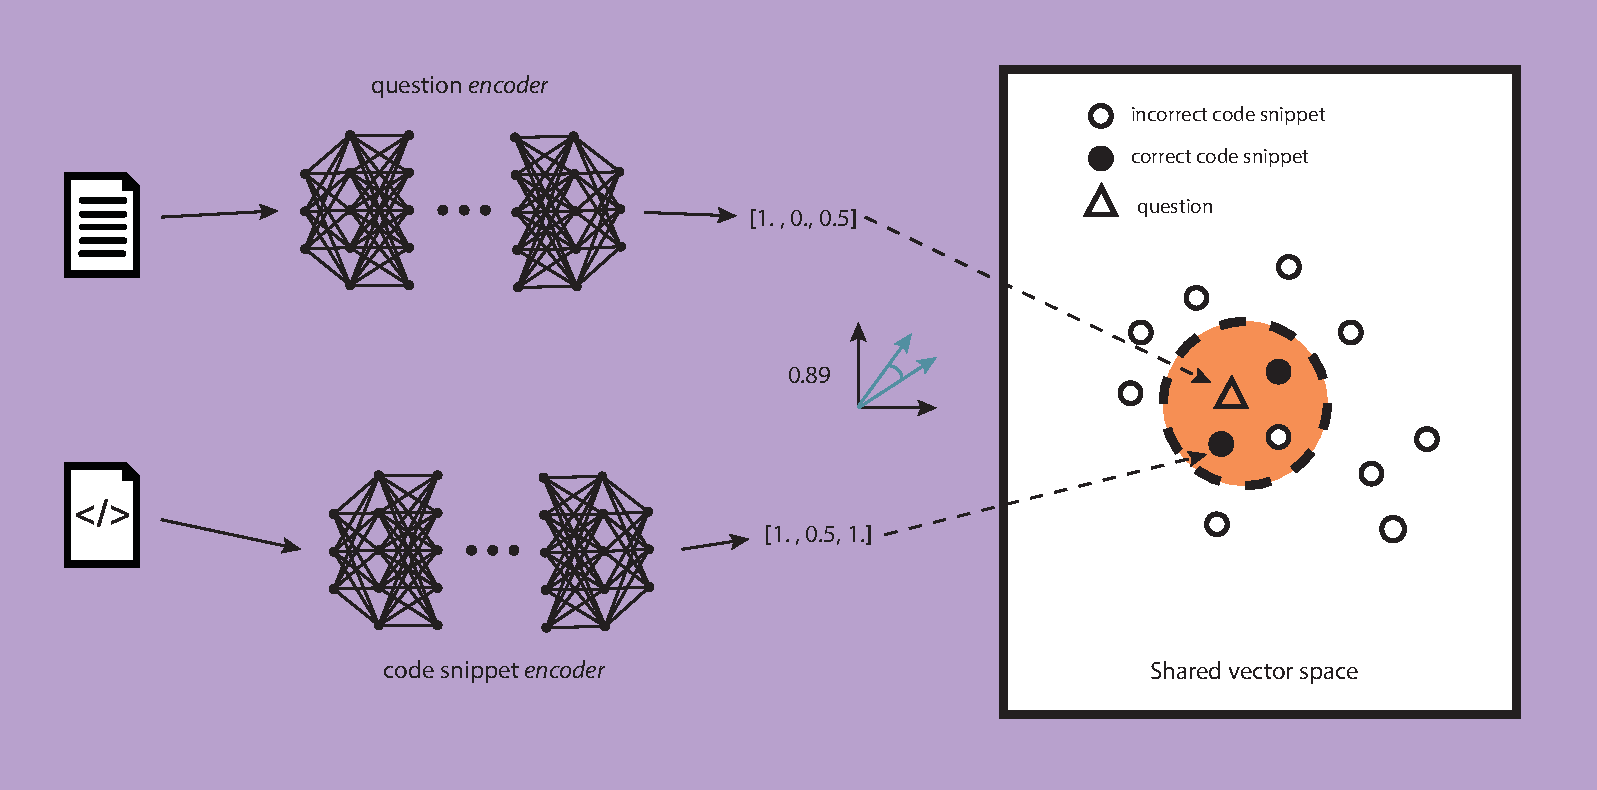
\includegraphics[width=0.45\textwidth]{figuras/joint_embedding-article.pdf}
  \caption{Illustration of \emph{joint embedding} technique for code retrieval. Two neural networks map a question and a code snippet into a common vector space. The distance between the vectors reflects the relevance of a code snippet to a question. Adapted from \cite{cambronero-deep-code-search-2019}.}
  \Description{None}
  \label{fig:joint-embedding}
\end{figure}


To apply joint embedding, 3 (three) items needs to be considered:

\begin{itemize}
    \item Word embedding
    \item Sentence embedding
    \item Joint embedding
\end{itemize}

Embedding refers to a continuous vector in a lower dimensional vector space. A function that maps an input to a continuous vector is called \emph{encoder}. So, given an input set $X$, an encoder function $F$ can be defined as \cite{cambronero-deep-code-search-2019}:

\begin{equation}
    F: X \to E
\end{equation}

For code retrieval, $X$ can be a set of questions or code snippets and $E$ is a set of continuous vectors or embeddings, such that $E \subset R^{d}$, where $d$ is the dimension. The main goal is to learn two encoders $F$ and $G$ that maps a question and a code snippet, respectively, into a common vector space, so that the distance between the vectors reflects the relevance of a code snippet to a question.

\section{Methodology}
\label{sec:methodology}

 In our work, we propose the use of convolutional neural networks to learn the sentence embedding, i.e., convolutional neural networks will encode the question and code snippet into a continuous vector in a shared vector space. In the following, we explain how words are embedded and what objective function we use, as the objective function tells how neural networks should approximate questions and code snippets.

\subsection{Word embedding}
\label{sec:word-embedding}

The words and terms of a question and code snippet must be encoded into a numeric vector. The most common encoder for words is \emph{word2vec}, which embeds a word into a continuous vector based on the distributional hypothesis. The distributional hypothesis says two words are similar if they appear together frequently in differents contexts \citep{Goodfellow-et-al-2016}. Context can be a sentence, paragraph, or document in NLP tasks. In our case, the context is questions and code snippets.

Word2vec has two strategies: continuous-bag-of-words (CBoW) and skip-gram. The main difference between them is that CBoW predicts a target word given context words, and skip-gram predicts the context words given a single word. According to \citet{mikolov2013distributed}, CBoW showed good results at syntactic tasks, e.g., finding a superlative of a word or identifying an adverb. At the same time, skip-gram presented a good performance for semantic tasks, e.g., finding the capital of a state or grouping feminine and masculine words. 

In our work, we opted for skip-gram as a semantic trait is preferable to a syntact one in our task. Semantic trait can help the neural networks to discriminate conditional clauses (e.g., \emph{if}, \emph{elsif}) and loop iteration (e.g. \emph{for}, \emph{while}), for example. Figure~\ref{fig:tsne-code-snippet-python} shows an application of word2vec in a Python related corpus. We can see the similarities between \emph{file}, \emph{write}, and \emph{open}, as \emph{set}, \emph{list}, and \emph{dict} based on the distance between them.

\begin{figure}[H]
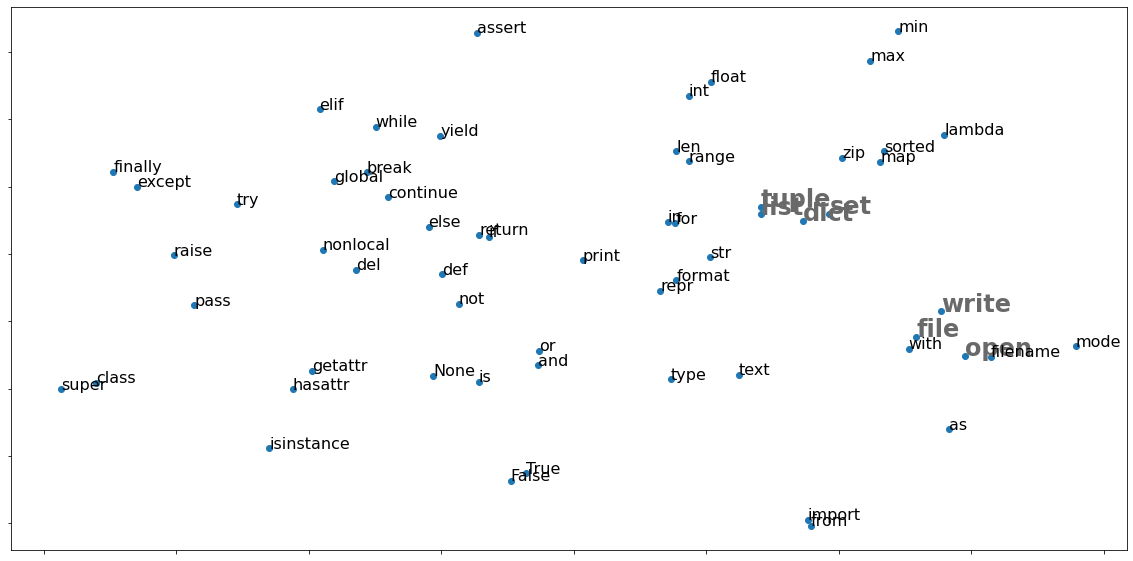
\includegraphics[width=0.45\textwidth]{figuras/code_tsne.png}
\caption{2D picture of continuous vectors of the 66 most frequent words from a Python corpus $V$. The illustration was generated by t-SNE, which allows 2D visualization from high-dimensional data. We applied word2vec with skip-gram and a parameter window $5$.}

\label{fig:tsne-code-snippet-python}
\end{figure}

\subsection{Sentence embedding}

We can combine the word embeddings to obtain a sentence embedding. We combine word embeddings by using convolutional neural networks. Convolutional neural networks showed good results at answer selection tasks in NLP---given a question and a set of answers, the model ranks the best answers. Convolutional networks prioritize local interactions (e.g., words nearby) and cannot capture long-range dependencies (e.g., distant words in a sentence). However, this issue is minimized for code retrieval since most questions and code snippets are short in length.

Given an sentence $\bm{x} = \{ \bm{x}(0), \bm{x}(1), . . ., \bm{x}(n - 1) \}$, such that $\bm{x}(i) \in \mathbb{R}^{d}$ is a continuous vector that represents the $i^{th}$ word of the sentence. Convolutional neural networks combine the elements of vector $\bm{x}$ by applying 2 basic operations:

\begin{itemize}
    \item Convolution operation
    \item \textit{Maxpool}
\end{itemize}

A convolution operation uses a filter $\bm{F}  = [\bm{F}(0),· · ·, \bm{F}(m - 1)]$, such that $\bm{F} \in \mathbb{R}^{m X d}$. The operation applies the filter in $m$ words (window size) to produce a new vector. Suppose $\bm{x}(i, i + j)$ refers to a concatenation of the vectors $\bm{x}(i), \bm{x}(i + 1), . . ., \bm{x}(i + j)$. If we apply $\bm{F}$ to $\bm{x}(i, i + m - 1)$, then we can calculate a new vector $\bm{c}(i)$ by:

\begin{equation}\label{eq:calc_convolution_ci}
    \bm{c}(i) = tanh \left[\left(\sum_{j=0}^{m - 1} \bm{x}(i + j)^{T}\bm{F}(j)\right) + b\right]
\end{equation}

In the equation~\ref{eq:calc_convolution_ci}, $\bm{F}$ and $b$ are learnable weights and bias, respectively. The convolution operation slides the filter $\bm{F}$ across the height of input $\bm{x}$ and computes the dot product between the entries of the filter and the input \cite{karpathy-course-cnn-2016}. The operation returns a feature map $\bm{c}$.

\begin{equation}
    \bm{c} = \{ \bm{c}(0), \bm{c}(1), . . ., \bm{c}(n - m) \} 
\end{equation}

The feature map (or activation map) contains the latent and most important features of a sentence. A convolutional neural network may contain thousands of filters, each one extracting specific \emph{m-gram} features (e.g., a filter of $m$ size 2 extracts bigram features). The quantity of feature maps is $|F|$, i.e., the number of filters. After the convolution operation, a pooling layer operates independently on every feature map resizing it spatially, using a max operation \cite{karpathy-course-cnn-2016}. The max operation is applied along the $axis=0$ to produce the final vector $\bm{o}$:

\begin{equation}
    \bm{o} = max\left(\left[\bm{c}_{1}, \bm{c}_{2}, . . ., \bm{c}_{|F|}\right], axis = 0\right)
\end{equation}

The max-pooling helps the convolutional neural networks to be translation invariant. Regardless of the word's position shift, the max-pooling selects the most relevant features and inserts it into the final vector \citep{tom-young:trends-deep-learning-nlp}. Figure~\ref{fig:cnn-steps-word-embedding} shows the results of each operation. We use the vector $\bm{o}$ as our sentence embedding, then $\bm{o}$ represents a question or a code snippet, in our case. 

\begin{figure}[H]
    \centering
    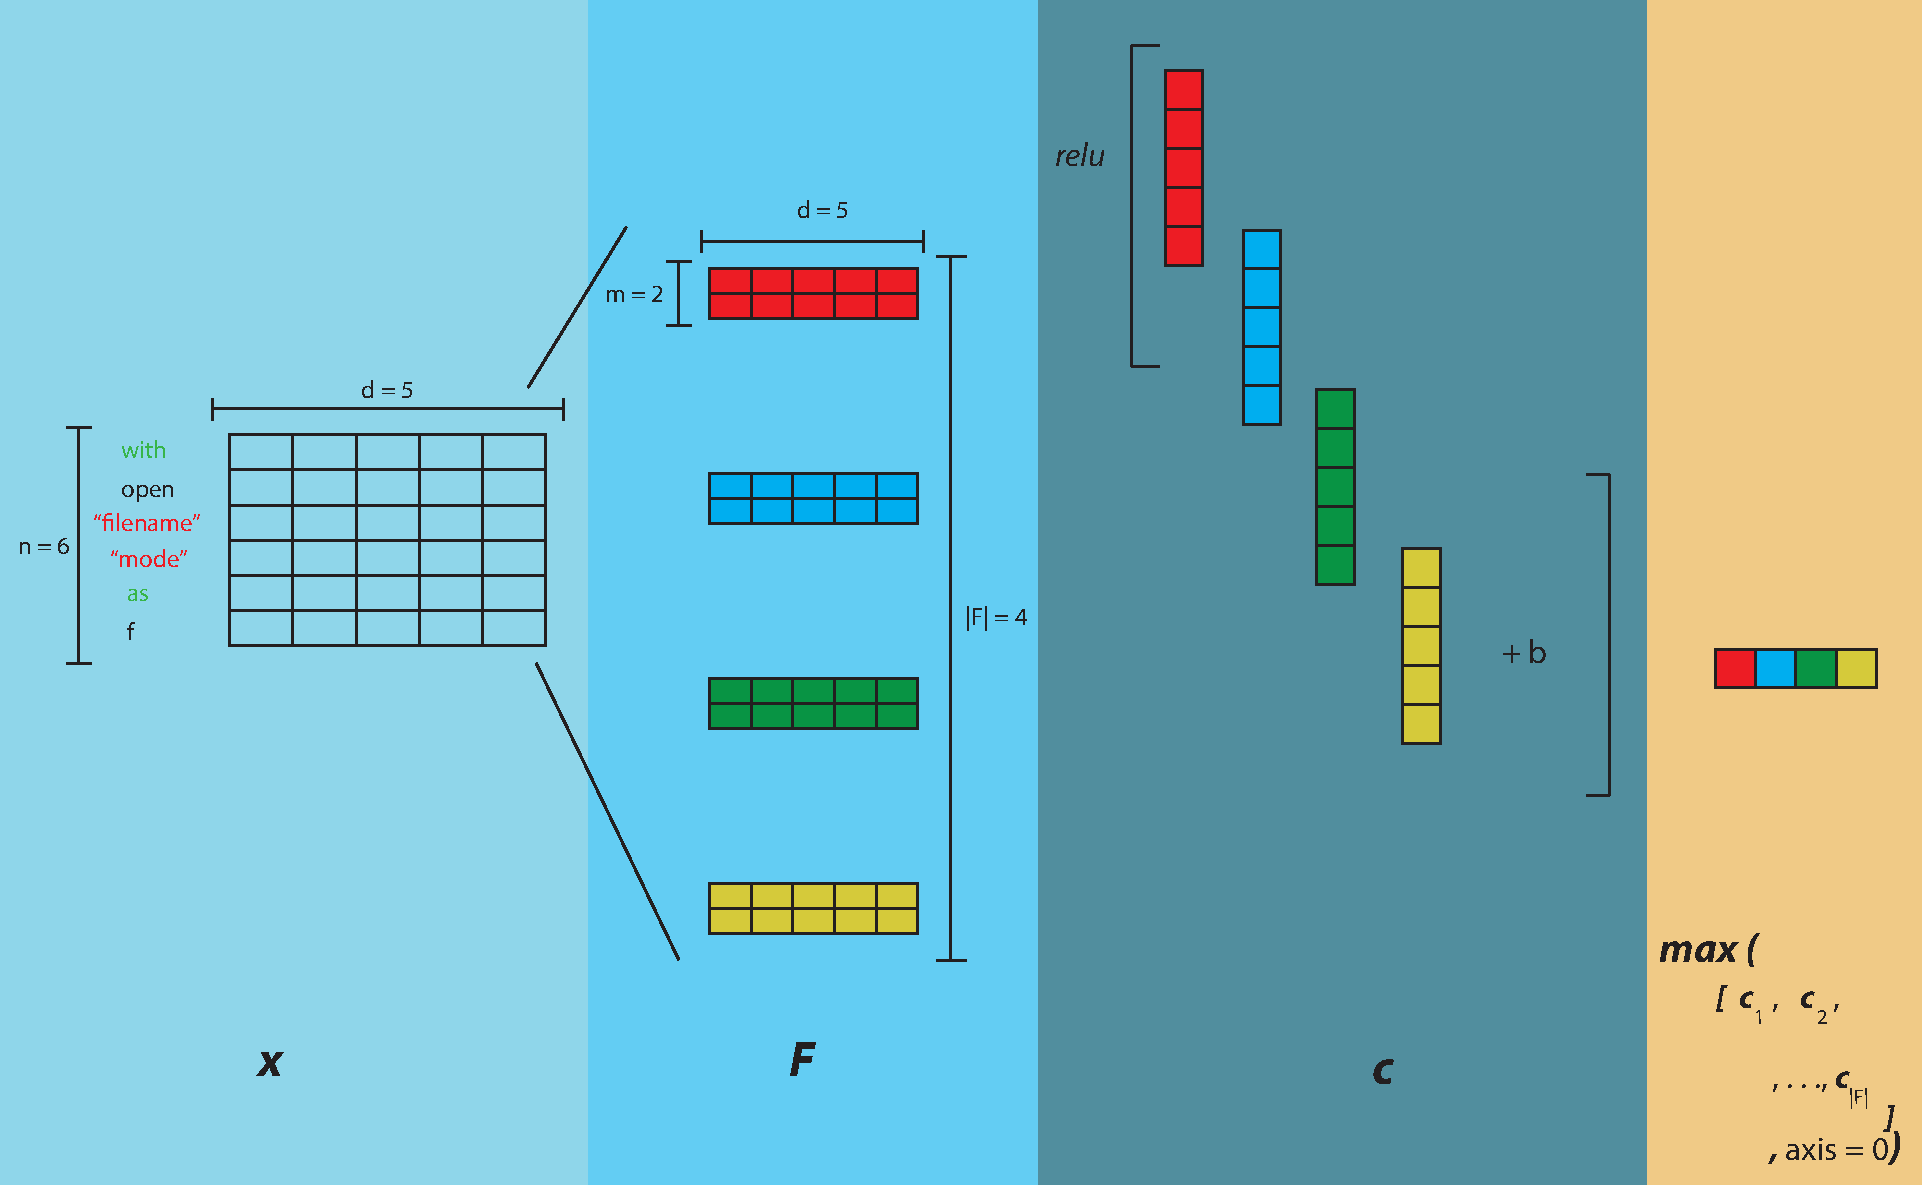
\includegraphics[width=0.45\textwidth]{figuras/cnn-steps-word-embedding-article.pdf}
    \caption{Schematic drawing of our Convolutional Neural Networks (CNN) operations. Our example shows 4 filters $\bm{F} \in \mathbb{R}^{m X d X f}$ with window size $m = 2$. We slide each filter across the height of the input $\bm{x} \in \mathbb{R}^{n X d}$, where $n = 6$ and $d = 5$, and computes the dot product between the entries of the filter and the input \cite{karpathy-course-cnn-2016}. It returns a feature map $\bm{c}$. In the end, a max pooling layer resizes every feature map spatially, obtaining the final vector $\bm{o}$. We use the vector $\bm{o}$ as our question and code snippet embedding. Adapted from \cite{zhang-guide-convolutional-cnn-embedding-ilustration:2015}.}
    \label{fig:cnn-steps-word-embedding}
\end{figure}

\subsection{Joint embedding}
\label{sec:joint-embedding}

In our work, we treat code retrieval as a ranking problem, where a model should rank relevant code in the top positions based on a developer's intent. To do so, we adopted an objective function that prioritizes the relative preference of the code snippets, instead of correct classification. In our case, the objective function helps the neural networks to separate the correct answers from incorrect ones during the training phase.

Given a question and code snippet set, $\mathbb{Q}$ and $\mathbb{C}$, our training input is composed of a triple $<\bm{q}, \bm{c^{+}}, \bm{c^{-}}>$, where $\bm{c^{+}} \in \mathbb{C}$ indicates a correct code snippet for a question $\bm{q} \in \mathbb{Q}$ and $\bm{c^{-}} \in \mathbb{C}$ its an incorret one sampled from the training data. We used the hinge loss as our objective function. Formally, for a triple $<\bm{q}, \bm{c^{+}}, \bm{c^{-}}>$, the definition of hinge loss is:

\begin{equation}
J = max(0, m - h_{\theta}(\bm{q}, \bm{c^{+}}) + h_{\theta}(\bm{q}, \bm{c^{-}}))
\end{equation}

$m$ is a margin and $h_{\theta}$ is a similarity function (e.g., \textit{cosine}). During the training phase, the goal is to minimize the cost function $J$. To obtain that, the model aims to satisfy the following condition: $h_{\theta}(\bm{q}, \bm{c^{+}}) - h_{\theta}(\bm{q}, \bm{c^{-}}) \geq m$. Then, the hinge loss function induces our model to score $c^{+}$ higher than $c^{-}$ for a given margin $m$. 

For the similarity function $h_{\theta}$, we used \emph{cosine}, such that $h_{\theta}(\bm{q}, \bm{c}) = \{h_{\theta}(\bm{q}, \bm{c}) \in \mathbb{R} | 0 \leq h_{\theta}(\bm{q}, \bm{c}) \leq 1$\} computes the similarity between the vector $\bm{q} \in \mathbb{Q}$ and $\bm{c} \in \mathbb{C}$. $0$ indicates orthogonality e $1$ indicates greater similarity \cite{keras-cosine-similarity-2019}. Given that our objective function aims to satisfy the following condition: $h_{\theta}(\bm{q}, \bm{c^{+}}) \geq h_{\theta}(\bm{q}, \bm{c^{-}}) + m$, our model groupw $\bm{c^{+}}$ and $\bm{q}$ nearby, while the vectors $\bm{c^{-}}$ would be far away (see Figure~\ref{fig:joint-embedding}). 

\section{Experiments}

In order to verify the efficacy of our approach and how it compares to a baseline and SOTA methods, we trained and evaluated all models on the same environment, following \citet{yao-2018} and \citet{ iyer-etal-2016-summarizing} experiment protocol. We compared the following models:

\begin{itemize}
    \item \emph{CoNCRA}: our proposed approach described in Section~\ref{sec:methodology}. We tried two variations of our approach, the Convolutional Neural Networks (CNN) and Shared CNN. Their difference is that Shared CNN shares the weights by learning the question and code snippet embeddings, while CNN learns different weights for each one.
    \item \emph{Embedding}: it is our baseline model. It is a simple architecture that applies a max-pooling layer to the word embeddings. 
    \item \emph{Unif}: it is the solution proposed by \citet{cambronero-deep-code-search-2019}. They used two distinct layers for the question and code snippet embedding. They applied an average pooling layer to word embedding to learn the question embeddings. For the code snippet, they used an attention mechanism, which applies a weighted average to each word embedding, ''giving attention'' to the most relevant word of the code.
\end{itemize}




We evaluated the models on the StaQC dataset, a systematically mined question-code dataset from Stack Overflow \cite{yao-2018}. The main difference of StaQC to other datasets is that it is composed of ''how-to-do-it'' questions, as most of the answers to those types of questions are straight. StaQC contains SQL and Python questions, but, in our preliminary experiments, we used Python questions only. Table~\ref{table:summary-training-data-yao-staqc} shows a summary of the StaQC dataset.

\begin{table}[h]
\centering
\begin{tabular}{ p{5cm} c c }
\hline
  & \multicolumn{2}{c}{\textbf{Question}}\\
\hline
\textbf{Code snippet} & \textbf{Python} & \textbf{SQL}  \\
\hline

$N_{1}$: Single code snippet in the answer description & $85.294$ & $75.637$ \\

$N_{2}$: Automatically annotated code snippets & $60.083$ & $41.826$ \\

$N_{3}$: Manually annotated code snippets & $2.169$ & $2.056$  \\

 \hline
 \textbf{Total} & $\bm{147.546}$ & $\bm{119.519}$\\
 \hline 
 
\end{tabular}
\caption{Summary of StaQC dataset \cite{yao-2018}. Questions from $N2$ sample ("Automatically annotated code snippets") may contain more than one code snippet per answer description. Some code snippets may not be a solution to the question. So, the authors proposed a framework to annotate the code snippets automatically and it could achieve an F1 score of $0,916$ and an accuracy of $0,911$.}
\label{table:summary-training-data-yao-staqc}
\end{table}

\begin{table}[h]
\centering
\begin{tabular}{ l r  }
 \hline
 \textbf{Sample} & \textbf{Quantity of pairs $<q_{i}, c_{i}^{+}>$}\\
 \hline
 $N_{2} = \text{Training}$ & $60.083$\\
 
 $N_{3} \supset \text{DEV}$ & $1.085$ \\
 
 $N_{3} \supset \text{EVAL}$ & $1.084$\\
 \hline
 \textbf{Total} & $\bm{62.252}$\\
 \hline
\end{tabular}
\caption{Summary of our training and evaluation samples. The samples are composed of a pair $<q_{i}, c_{i}^{+}>$, where $q_{i}$ its a question and $c_{i}^{+}$ its a code snippet annotated as solution. We spplited the manually annotated dataset in two parts: DEV and EVAL, according to \cite{iyer-etal-2016-summarizing} procedure. }
\label{table:training-sample-division}
\end{table}

All models were trained on sample $N2$ (see Table~\ref{table:summary-training-data-yao-staqc} and Table~\ref{table:training-sample-division}), because 27\% of the questions contain more than one answer annotated, leading to more variance in our training dataset. The training and evaluation follow the \citet{iyer-etal-2016-summarizing} procedure, where the model is evaluated on a manually annotated dataset each epoch according to a Mean Reciprocal rank (MRR). The MRR tells if a model ranked the annotated answer in higher positions, i.e., higher values for MRR indicate the accepted answers were ranked in the top positions.

For the training phase, we split 70\% of $N2$ sample for training and 30\% for validation. We run the models for 500 epochs and stop early if the training loss ($J$) is less than $0.0001$ or the validation loss does not improve after 25 consecutive epochs. For the final evaluation, we choose the best model of the training phase according to MRR and run it for 20 iterations in the $N3$ sample (see Table~\ref{table:training-sample-division}). The final result is the average of the MRR for each pair $<q_{i}, c_{i}^{+}>$ of $N3$ and other 49 distractors $c_{j}$, which were selected randomly from the training sample, such that $c_{i}^{+} \neq c_{j}$.

We provide the source code for our preliminary experiments in the following repository: \url{https://github.com/mrezende/concra}. The repository contains our proposed model, the baseline ones, training, and evaluation source code. We also provide the original and pre-processed dataset. The source code is written in Python, version 3.6.9, and we used the libraries Keras (version 2.2.4-tf) and TensorFlow (1.15.2). The tests were all conducted in the Colab platform\footnote{\url{https://colab.research.google.com/}}.

\subsection{Results}

 Table~\ref{table:resultados} compiles the final results after 20 runs on the $N3$ sample. Shared CNN with 4000 filters got the best results (row D3 and F3). Our proposed architecture achieved an MRR score 5\% higher on average than the best result obtained by Unif (row B1), which can be considered an state-of-the-art approach. Our MRR result is 11\% higher than the baseline model (row A1). 

\begin{table*}[t]
\centering
\begin{tabular}{ p{1cm} p{6cm} >{\raggedleft\arraybackslash}p{4cm} >{\raggedleft\arraybackslash}p{4cm} }
 \hline
    & & \multicolumn{2}{c}{\textbf{Results}}\\
 \hline
 & \textbf{Models} & \textbf{MRR} & \textbf{TOP-1}\\
 \hline
 A1 & Embedding (m = $0.1$) & $0.637$& $0.493 \pm 0.009$\\
 
 \hline
 
 B1 & Unif (m = $0.2$) & $0.675 \pm 0.006$ & $0.539 \pm 0.009$\\
 
 \hline
 
 C1 & CNN / F = 1000 & $0.669 \pm 0.006$ & $0.527 \pm 0.012$\\
 
 C2 & CNN / F = 2000 & $0.673 \pm 0.007$ & $0.531 \pm 0.012$\\
 
 C3 & CNN / F = 4000 & $0.687 \pm 0.006$ & $0.553 \pm 0.011$\\
 
 \hline
 
 D1 & Shared CNN / F = 1000 & $0.678 \pm 0.007$ & $0.548 \pm 0.012$\\
 
 D2 & Shared CNN / F = 2000 & $0.694 \pm 0.008$ & $0.565 \pm 0.012$\\
 
 D3 & Shared CNN / F = 4000 & $0.700 \pm 0.004$ & $0.569 \pm 0.009$\\
 
 \hline
 
 E1 & CNN with BN / F = 1000 & $0.682 \pm 0.007$ & $0.543 \pm 0.012$\\
 
 E2 & CNN with BN / F = 2000 & $0.689 \pm 0.006$ & $0.553 \pm 0.011$\\
 
 E3 & CNN with BN / F = 4000 & $0.688 \pm 0.006$ & $0.553 \pm 0.011$\\
 
 \hline
 
 F1 & Shared CNN with BN / F = 1000 & $0.690 \pm 0.008$ & $0.553 \pm 0.015$\\
 
 F2 & Shared CNN with BN / F = 2000 & $0.700 \pm 0.007$ & $0.573 \pm 0.012$\\
 
 F3 & Shared CNN with BN / F = 4000 & $0.701 \pm 0.008$ & $0.577 \pm 0.015$\\
 
\hline
\end{tabular}
\caption{The experimental results of EVAL sample for Embedding, Unif, and our two CNN variations: CNN and Shared CNN. \emph{m} refers to the margin loss of the hinge loss function (lines A1 and B1). \emph{F} indicates the number of filters. BN its an acronym of Batch Normalization. Our CNN architecture used a margin loss $m = 0.05$ and a window size $2$.}
\label{table:resultados}
\end{table*}

As presented in Table~\ref{table:resultados}, an increase in the number of filters resulted in a better performance for CNN, as the model capacity and the number of extracted features grow (row D3 and F3). 
We tried different margin loss (see Section~\ref{sec:joint-embedding}). CNN got the best results with  $0.05$, while Unif and Embedding got better results with $0.2$ and $0.1$, respectively. 

We verified that shared weights models (row D and F) got better results than independently weights ones (row C and E). One reason is that the optimizer of independent weights architecture has to learn the double of parameters, increasing the learning difficulty \cite{feng-2015}. We also tried a batch normalization technique to avoid overfitting and help our models to learn quickly and a more stable way, but only CNN and Shared CNN got better results. For Unif and Embedding, it did not improve the performance at all. 

The Figure~\ref{fig:histogram-mrr} illustrates the MRR (Mean Reciprocal Rank), showing the first position of the annotated code snippet during the final evaluation.

\begin{figure}[H]
    \centering
    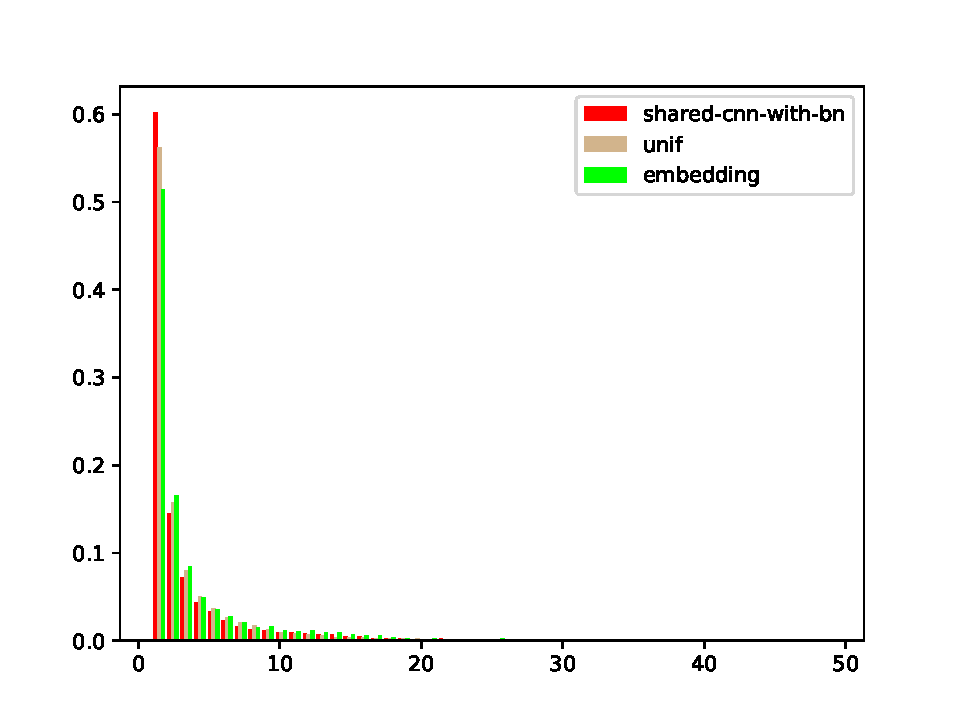
\includegraphics[width=0.45\textwidth]{figuras/histogram.pdf}
    \caption{Histogram of the firsts positions observed for the annotated code snippet during the final evaluation. The labels \emph{shared-cnn-with-bn}, \emph{unif} and \emph{embedding} refer to lines F3, A1 e B1, respectively, in the Table~\ref{table:resultados}.}
    \label{fig:histogram-mrr}
\end{figure}


Both CNN and Unif ranked the code snippets among the first three positions in 75\% of cases. We got a TOP-1 accuracy of 60\%, i.e., we ranked the relevant code snippet first place in 60\% of cases. Unif and Embedding got a TOP-1 accuracy of almost 50\%. However, one thing to note is that MRR considers only the annotated code snippet position. If the model shows up another code snippet, which correctly answers the question, our metric does not take it into account and the model is penalized. 

\subsection{Threats to validity}

We trained the models on the StaQC dataset, a systematically mined question code dataset. The authors used neural networks to annotate the code snippet and trained it on a manual dataset. In our case, we trained the models on the automatically annotated corpus and evaluated on the manual ones. To mitigate bias, we adopted the \citet{iyer-etal-2016-summarizing} procedure for training and evaluation.

\section{Related Work}

We summarized the difference between our work and related work in Table~\ref{table:summary-joint-embedding-related-work}. Most works differ on how they combine the words embeddings to obtain a sentence embedding. Recent works (row E and F) used Skip-gram (see Section~\ref{sec:word-embedding}) and adopted simpler archictectures for sentence embedding than previous work (row C and D).  

Previous work (from row D to F) that used GitHub's data extracted the methods from the source code and matched them to docstring descriptions. Work that used Stack Overflow  (from row A to C) paired question title to the code snippet of the accepted answer. For the search corpus, some works (from row D to F) adopted a GitHub corpus with milions of pieces of code, while others  (from row A to C) retrieved code snippet from a small sample of 50 code snippets randomly selected. The studies (from row A to G) are commonly evaluated using questions collected from Stack Overflow. 

Although, our architecture are more complex, require more parameters and time to train, than \citet{cambronero-deep-code-search-2019} (row F) architecture (SOTA), we think it's not a overhead, as we can train our model offline. We matched question title to code snippets collected from Stack Overflow following \citet{Allamanis-bimodal-source-code-natural-language:2015} and \citet{iyer-etal-2016-summarizing} (row A and B) work. 


\begin{table}[t]
\centering
\begin{tabular}{ p{0.1cm} p{2cm} p{1.5cm} p{1.5cm} p{1.5cm} }
 \hline
 & \textbf{Work} & \textbf{Feature} & \textbf{Word Embedding} & \textbf{Sentence Embedding} \\
 \hline
A & \citet{Allamanis-bimodal-source-code-natural-language:2015} & Token / Parse Tree & Probabilistic Model & Average / Context matrix  \\

B &\citet{iyer-etal-2016-summarizing} & Token & One-hot encoding & LSTM with attention mechanism  \\

C &\citet{Chen-bi-variational-autoencoder:2018} & Token & Bi-VAE & Bi-VAE, Average and MLP  \\

D &\citet{Gu-deep-code-search:2018} & Token / Method name, API invocation and Token & bi-LSTM & Max-pooling / Max-pooling and MLP   \\

E &\citet{Sachdev-neural-code-search:2018} & Token & Skip-gram & Average / TF-IDF   \\

F &\citet{cambronero-deep-code-search-2019} & Token & Skip-gram & Average / Attention   \\

G & \textit{Our work} & \textit{Token} & \textit{Skip-gram} & \textit{CNN}   \\

 \hline
\end{tabular}
\caption{Summary of related joint embedding work. The column \emph{Feature} refers to question and code representation. Different approachs for a question and code snippet are separated by slash (''/''), showing the question method first followed by the code snippet technique. Adapted from \cite{yan-benchmark-code-search-information-retrieval-deep-learning:2020}.}
\label{table:summary-joint-embedding-related-work}
\end{table}



\section{Conclusion}

According to results, our model achieved an MRR score 5\% higher on average than Unif, actual state-of-the-art. We could rank the most relevant code snippet among the first 3 (three) positions in 78\% of cases. Our technique achieved a TOP-1 accuracy of 60\%, while the other techniques got 50\%. 

The results seem promising, and we plan a further investigation to see if our model is invariant to other datasets. We will also investigate transfer learning, e.g., checking if a model trained on a Stack Overflow dataset (curated corpus) can find relevant code snippets in a GitHub corpus (non-curated one). Our approach is based on an NLP technique proposed by \citet{feng-2015}, and future work may use transformers and autoencoders, as those techniques showed good results in many NLP tasks. 

%%
%% The next two lines define the bibliography style to be used, and
%% the bibliography file.
\bibliographystyle{ACM-Reference-Format}
\bibliography{sample-base}

%%
%% If your work has an appendix, this is the place to put it.


\end{document}
\endinput
%%
%% End of file `sample-sigconf.tex'.
